\documentclass[../notes.tex]{subfiles}

\pagestyle{main}
\renewcommand{\chaptermark}[1]{\markboth{\chaptername\ \thechapter\ (#1)}{}}
\setcounter{chapter}{4}

\begin{document}




\chapter{Even More Catalytic Processes}
\section{Lecture 18: Olefin Polymerization}
\begin{itemize}
    \item \marginnote{5/10:}Another huge industrial-scale reaction
    \item The Great Pacific Garbage Patch is largely composed of plastics made by this process.
    \begin{itemize}
        \item Plastics get a bad rep, but they are a remarkable material.
        \begin{itemize}
            \item We can melt them, form them, and they have durability properties.
        \end{itemize}
        \item However, because of their environmental impact, a big thing in chemistry is the pursuit of materials with similar properties that are biodegradable.
        \item Inorganic chemistry plays a large role in their synthesis.
        \item In 2008, the US alone made 58.3 million metric tons of polyethylene and 17 million metric tons of polypropylene.
    \end{itemize}
    \item General form:
    \begin{figure}[h!]
        \centering
        \schemestart
            \chemfig{R-[:30]=_[:-30]}
            \arrow{->[\small cat]}
            \chemleft{(}
                \chemfig{-[:30,0.5]-[:-30](-[6]R)-[:30,0.5]}
            \chemright{)_n}
        \schemestop
        \caption{The general form of olefin polymerization.}
        \label{fig:olefinPolymerization}
    \end{figure}
    \begin{itemize}
        \item If $\ce{R}=\ce{H}$, we have polyethylene.
        \item If $\ce{R}=\ce{Me}$, we have polypropylene.
    \end{itemize}
    \item This is a thermodynamically favorable, exothermic reaction since $\pi$ bonds are weaker than $\sigma$ bonds.
    \item The catalyst is typically \ce{Ti}, \ce{Zr}, \ce{Hf}, \ce{Cr} (early Group 4 transition metals). Sometimes we use \ce{Fe}, \ce{Co}, \ce{Ni}, and \ce{Pd} (these are a bit more specific).
    \item Most of the materials that mediate this catalysis are called Ziegler-Natta catalysts.
    \begin{itemize}
        \item These are heterogeneous, even though they operate via the same kind of catalytic cycle that homogeneous systems use.
        \item Nobel prize (1963).
    \end{itemize}
    \item Polymer terms:
    \item \textbf{Number averaged molecular weight}: The quantity $\frac{\sum N_xM_x}{\sum N_x}$, where $N_x$ is the number of chains with $x$ monomers and $M_x$ is the molecular weight of a chain with $x$ monomers. \emph{Also known as} $\bm{M_N}$.
    \item \textbf{Weight averaged molecular weight}: The quantity $\frac{\sum N_xM_x^2}{\sum N_xM_x}$. \emph{Also known as} $\bm{M_w}$.
    \item \textbf{Molecular weight distribution}: The quantity $\frac{M_w}{M_N}$. \emph{Also known as} \textbf{polydispersity index}, \textbf{PDI}.
    \begin{itemize}
        \item 1 is perfect. This means that you only have one type of chain.
        \item 1.1 is good.
        \item Above 1.5 is getting ill-defined.
    \end{itemize}
    \item Stereochemistry:
    \begin{itemize}
        \item Normally, the methyl groups in polypropylene all insert on the same side, but if one misinserts, then it faces the other direction.
        \item If the catalyst corrects itself and continues on inserting in the original direction, this is \textbf{site control}.
    \end{itemize}
    \item \textbf{Site control}: The catalyst controls the insertion.
    \begin{itemize}
        \item More specifically, the direction the methyl groups point is controlled by the catalyst.
    \end{itemize}
    \item \textbf{Chain end control}: One misinsertion causes the ensuing insertions to face the same way as the last inserted methyl group.
    \begin{itemize}
        \item More specifically, the direction the methyl groups point is controlled by the last inserted methyl group.
    \end{itemize}
    \item Mechanism:
    \begin{equation*}
        \ce{L_nMR2 ->[LA][-LAR^-] L_nMR+ ->[||] L_nM---R ->[] L_nM-H}
    \end{equation*}
    \begin{itemize}
        \item The three steps are activation, growth, and termination.
        \item LA stands for Lewis acid. The lewis acid activates the catalyst by abstracting an anionic Lewis acid species.
        \item Olefin insertion grows the polymer.
        \item $\beta$-\ce{H} elimination is the simplest way to terminate the chain, even though there are several possibilities.
    \end{itemize}
    \item Activation:
    \begin{itemize}
        \item \ce{L_nMCl2 ->[AlR3/MAO] L_nMMe2 ->[AlR3/MAO][-AlR4^-] L_nMe+}.
        \item \ce{L_nMCl2 ->[AlR3/MAO] L_nMMe2 ->[BAr^F{}_3][-MeBAr^F{}_4-] L_nMe+}.
        \item \ce{L_nMCl2 ->[AlR3/MAO] L_nMMe2 ->[HBAr^F{}_4][-CH4] L_nMe+}.
        \item MAO is methylated aluminum oxide.
        \begin{itemize}
            \item An ill defined, amorphous gunk with some oxygens created by adding a pinch of water to \ce{AlMe3}.
            \item A cheap reagent that people chuck into their catalyst mixture.
            \item Functions:
            \begin{enumerate}
                \item Alkylating agent.
                \item Activator (pulls off methyls to generate cationic species).
                \item Scavenger for water (primarily) and oxygen.
            \end{enumerate}
        \end{itemize}
        \item The fluorinated aryl borates are really good because they're very weakly coordinating, and we really want an open coordination site.
    \end{itemize}
    \item Chain growth:
    \begin{itemize}
        \item \ce{MR(||) -> M---R ->[||] M(||)(---R) -> M---R -> -> ->}.
        \item This is called the Cossee Arlman mechanism.
        \item Sterics determine the rates: Ethylene $>$ propylene $>$ substituted olefins $>$ disubstituted olefins $\approx$ geminal disubstituted olefins $>>>$ trisubstituted or tetrasubstituted olefins.
    \end{itemize}
    \item Termination:
    \begin{itemize}
        \item How you get variability in chain lengths.
        \item Control it by adding a chain-transfer reagent (a specific terminating reagent). Examples include\dots
        \begin{itemize}
            \item \ce{H2}: \ce{L_nM-pl ->[H2] L_nM-H + H-pl}, where \ce{pl} is a polymer\footnote{Be aware that Anderson uses a capital P in a circle.}.
            \item $\beta$-\ce{H} elimination: \ce{L_nM---pl -> L_nM(H)(||pl) -> L_nM-H + =-pl}.
            \item $\beta$-\ce{H} abstraction: \ce{M(||)(---pl) -> M(Et)(||pl) -> MEt + =-pl}.
        \end{itemize}
    \end{itemize}
    \item The relative rates of growth vs. determination dictate the type of material we get.
    \begin{itemize}
        \item $K_p$ is the rate of growth/propogation; $K_t$ is the rate of termination.
        \item $K_p$ vs. $K_t$ dictates the product.
        \item $K_p>>>K_t$ yields high molecular weight polymers.
        \item $K_p\approx K_t$ (within the same order of magnitude) yields oligomers.
        \begin{itemize}
            \item The geometric weight distribution of oligomers is called a \textbf{Schultz-Flory distribution}.
        \end{itemize}
        \item $K_t>>K_p$ yields dimers exclusively.
        \begin{itemize}
            \item This can be valuable if you just want to transform ethylene into butadiene (a higher value product), for instance.
        \end{itemize}
    \end{itemize}
    \item Types of polyethylene.
    \begin{figure}[h!]
        \centering
        \begin{subfigure}[b]{0.3\linewidth}
            \centering
            \chemfig{[:54]M*5([,1.25]-N(-[,0.8]R)=-=N(-[,0.85]R)-)(-[5]X)(-[7]X)}
            \caption{LDPE catalysts.}
            \label{fig:catalysts-polyethylenea}
        \end{subfigure}
        \begin{subfigure}[b]{0.3\linewidth}
            \centering
            \chemfig{M?(-[3]Cp(-[1]R)-[5]Si(-[3])(-[5])-[7]N?R)(-[1]X)(-[7]X)}
            \caption{LLDPE catalysts.}
            \label{fig:catalysts-polyethyleneb}
        \end{subfigure}
        \caption{Polyethylene-type catalysts.}
        \label{fig:catalysts-polyethylene}
    \end{figure}
    \item A perfect zig-zag chain is HDPE (high density polyethylene).
    \begin{itemize}
        \item High melting point.
        \item Crystalline.
        \item Example uses: Helmets for army soldiers, bulletproof plastics.
        \item Usually formed with Ziegler-Natta catalysis:
        \begin{itemize}
            \item \ce{TiCl_x + AlR_x ->} a heterogeneous catalyst that's super active ($>\SI{e9}{\kilo\gram}$ of polymer per gram of catalyst).
            \item Note that $x=3$ or 4.
            \item Alternate catalysts: \ce{Cr^{III} + {silica} ->[O2, $\Delta$] CrO4 ->[||]} reduced Cr center (the active catalyst).
        \end{itemize}
    \end{itemize}
    \item A mess with a ton of branching is LDPE (low density polyethylene).
    \begin{itemize}
        \item Lower melting point.
        \item Often made by radical processes.
        \item Also made by late transition metal catalysts, where there's less control over chain growth:
        \begin{itemize}
            \item Square planar, $d^8$, $16\,\e[-]$ species.
            \item Example metal centers: \ce{Ni}, \ce{Pd}.
            \item High rates of $\beta$-\ce{H} elimination leads to chain walking and branching.
        \end{itemize}
    \end{itemize}
    \item Longer chain with a few branches is linear low-density polyethylene (LLDPE).
    \begin{itemize}
        \item Transition metal catalyzed.
        \item Formed from a mixture of ethylene and substituted olefins or a controlled rate of branching from catalysts.
        \item Catalysts:
        \begin{itemize}
            \item Constrained geometry catalysts.
            \item Example metal centers: \ce{Ti}, \ce{Zr}, \ce{Hf}.
        \end{itemize}
    \end{itemize}
    \item Polyethylene gives a single chain, but polypropylene can be chiral depending on the orientation of the methyl groups. The orientation defines \textbf{tacticity}.
    \item \textbf{Isotactic} (polypropylene): All methyl groups are pointed in the same direction.
    \begin{itemize}
        \item The most crystaline, highest melting point material.
    \end{itemize}
    \item \textbf{Atactic} (polypropylene): Every methyl group is random.
    \begin{itemize}
        \item The least crystaline, lowest melting point material.
    \end{itemize}
    \item \textbf{Syndiotactic} (polypropylene): Every methyl group alternates.
    \begin{itemize}
        \item Pretty highly ordered.
    \end{itemize}
    \item \textbf{Hemiisotactic} (polypropylene): Every other methyl group points the same direction; the remaining ones are random.
    \item \textbf{Stereoblock} (polypropylene): Alternating blocks of isotactic polypropylene.
    \item Controlling stereochemistry:
    \begin{itemize}
        \item Relies on the fact that propylene is pro-chiral.
        \item Si (pro-S) and Re (pro-R) faces.
        \item Catalyst symmetry controls tacticity.
    \end{itemize}
    \item Catalyst types:
    \begin{figure}[h!]
        \centering
        \begin{subfigure}[b]{0.3\linewidth}
            \centering
            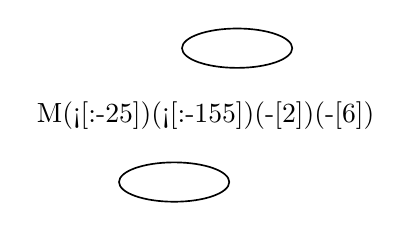
\begin{tikzpicture}
                \node {\chemfig{M(<[:-25]\coordsite)(<[:-155]\coordsite)(-[2])(-[6])}};
    
                \filldraw [fill=white,semithick] (0.4,0.85) ellipse (7mm and 2.5mm);
                \draw [semithick] (-0.4,-0.85) ellipse (7mm and 2.5mm);
            \end{tikzpicture}
            \caption{$C_2$ symmetry.}
            \label{fig:catalysts-polypropylenea}
        \end{subfigure}
        \begin{subfigure}[b]{0.3\linewidth}
            \centering
            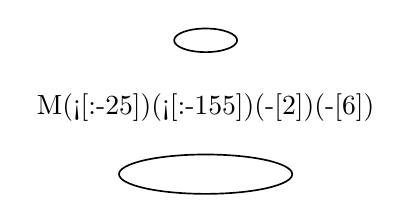
\begin{tikzpicture}
                \node {\chemfig{M(<[:-25]\coordsite)(<[:-155]\coordsite)(-[2])(-[6])}};
    
                \filldraw [fill=white,semithick] (0,0.85) ellipse (4mm and 1.5mm);
                \draw [semithick] (0,-0.85) ellipse (1.1cm and 2.5mm);
            \end{tikzpicture}
            \caption{$C_s$ symmetry.}
            \label{fig:catalysts-polypropyleneb}
        \end{subfigure}
        \begin{subfigure}[b]{0.3\linewidth}
            \centering
            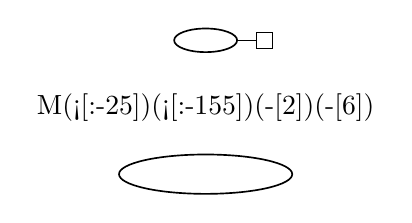
\begin{tikzpicture}
                \node {\chemfig{M(<[:-25]\coordsite)(<[:-155]\coordsite)(-[2])(-[6])}};
    
                \filldraw [fill=white,semithick] (0,0.85) ellipse (4mm and 1.5mm);
                \draw (0.4,0.85) -- ++(0.25,0) -- ++(0,0.1) -- ++(0.2,0) -- ++(0,-0.2) -- ++(-0.2,0) -- ++(0,0.1);
                \draw [semithick] (0,-0.85) ellipse (1.1cm and 2.5mm);
            \end{tikzpicture}
            \caption{$C_1$ symmetry.}
            \label{fig:catalysts-polypropylenec}
        \end{subfigure}
        \caption{Polypropylene-type catalysts.}
        \label{fig:catalysts-polypropylene}
    \end{figure}
    \begin{itemize}
        \item Most well worked out for metallocenes.
        \item In Figure \ref{fig:catalysts-polypropylene}, boxes are open coordination sites; circles are space-filling ligands.
        \item Differences help dictate tacticity.
        \item $C_2$: Both binding sites are the same.
        \begin{itemize}
            \item Steric clashing forces the olefin to point in inverted ways; but because the polymer switches sides, this leads to consistency in the direction the methyl is added.
            \item Generates isotactic polypropylene.
            \item Si-face selective.
            \item Example: A diindene metallocene.
        \end{itemize}
        \item $C_s$: Binding sites are enantiomers.
        \begin{itemize}
            \item Generates syndiotactic polypropylene.
            \item Two enantiotopic sites will alternate.
            \item Example: A metallocene with Cp on top and fluorene on bottom.
        \end{itemize}
        \item $C_1$: Binding sites are diastereomers.
        \begin{itemize}
            \item Generates hemiisotactic polypropylene.
            \item Example: A metallocene with \ce{Cp-R} on top and fluorene on bottom.
        \end{itemize}
    \end{itemize}
    \item To make this work, the \ce{Cp} rings are often tethered to prevent rotation.
    \begin{itemize}
        \item However, rotation can be harnessed to make stereoblock copolymers.
    \end{itemize}
    \item Note that stereoblock copolymers can also be synthesized with two isotactic catalysts, relying on chain transfer.
    \item Late-metals: Chain walking.
    \begin{itemize}
        \item A chain can grow or it can chain walk (do $\beta$-\ce{H} elimination followed by a $2,1$-insertion).
        \item If it chain walks, we'll create a branch.
    \end{itemize}
    \item We see this with late metals.
    \begin{itemize}
        \item Early metals are terrible backbonders, so they will prefer to be on the alkyl side of the equilibrium.
        \item Late metals can backbond, and will more readily form an olefin adduct (a necessary intermediate to chain walking).
    \end{itemize}
    \item Thus, we use late metals\dots
    \begin{itemize}
        \item Because sometimes we want branching, specifically finely tuned branching to a certain degree.
        \begin{itemize}
            \item Recall that random branching can be achieved via a radical mechanism.
        \end{itemize}
        \item SHOP process:
        \begin{itemize}
            \item We react ethylene with a nickel PO-type catalyst (a nickel catalyst with a bidentate ligand that chelates through a phosphorous and an oxygen), an enolate, or related phosphorous/oxygen based donors.
            \item This creates olefin-terminating oligomers. This doesn't use chain walking, but rather the chain transfer process, which is much faster with late metals.
            \item Products: \ce{C4{-}C8} ($41\%$), \ce{C10{-}C18} ($40.5\%$), and \ce{C_{20+}} ($18.5\%$).
            \item The short ones and the long ones can be combined with \ce{Mo2O3/Al2O3} to do olefin metathesis, yielding internal and terminal olefins.
            \item Then, throwing in the medium-length ones and treating with \ce{HCo(CO)4} (our hydroformylation catalyst) and syn gas yields terminal aldehydes, which with enough hydrogen can give us terminal alcohols, which are commodity chemicals.
        \end{itemize}
    \end{itemize}
    \item Oligomerization mechanism:
    \begin{figure}[H]
        \centering
        \schemestart
            \chemfig{M-H}
            \arrow{->[\small\subscheme{2\arrow{0}[,0.1]\chemfig{=[1]}}]}
            \chemfig{M(-[:30]-[:-30])(-[7]\phantom{i}-[1,0.4,,,white]=[5])}
            \arrow
            \chemfig{[:-30]M*6(------)}
            \arrow[,1.1]
            \chemfig{M?(-[2]\phantom{i}-[4,0.4,,,white]=-[::-30,1]-[::-50,0.9]-[::-70,0.8]?)(-[6]H)}
            \arrow{-U>[][*{0.-150}\small\chemfig{-[:30]-[:-30]=^[:30]}][][][135]}[-90]
            \chemfig{M^{\mathit{n}-2}(-[5]\phantom{i}-[3,0.4,,,white]=[7])(-[7]\phantom{i}-[5,0.4,,,white]=[1])}
            \arrow[180]
            \chemfig{M*3([:-100]---)*3([:-140]---)}
            \arrow[90,1.3]
        \schemestop
        \caption{Oligomerization mechanism.}
        \label{fig:mechanism-oligomerization}
    \end{figure}
    \begin{itemize}
        \item A metathesis-like process.
        \item Example with nickel.
    \end{itemize}
    \item Polar monomer incorporation.
    \begin{itemize}
        \item One of the standing grand challenges in olefin polymerization.
        \item Incorporating vinyl chlorides, vinyl ethers, vinyl esters, vinyl nitriles, etc.
        \item We can do this with radical polymerizations, but there's no stereocontrol here.
        \item PVC (pipe) is polyvinylchloride (robust, a great material, but opaque).
        \begin{itemize}
            \item It's melting point would be even higher if we could make it isotactic (and it would be clear, which could potentially have applications).
        \end{itemize}
        \item The challenge with early metals is that if you $\beta$-\ce{Cl} eliminate, the \ce{M-Cl} bond will be too strong to break and reinsert the chloride. This kills the catalysis.
        \begin{itemize}
            \item Additionally, the groups on the polymer adjacent to the metal center can donate to it, making the polymer a kind of chelating ligand and preventing olefin insertion. This also kills the catalysis.
        \end{itemize}
        \item Late metals are less halo/oxo-philic, which makes them better at incorporating these monomers.
    \end{itemize}
\end{itemize}



\section{Office Hours (Anderson)}
\begin{itemize}
    \item Chain walking is when the metal bonds to a $\sigma$ bond, moves to an adjacent carbon, moves to a double bond next, and on and on.
    \begin{itemize}
        \item The terminal olefins are sterically favored, even though the internal ones are typically thermodynamically favored.
        \item Early metals typically make linear polyolefins, while late metals prefer branched ones.
    \end{itemize}
    \item What is the difference between a Chatt, distal, and alternating mechanism?
    \begin{itemize}
        \item Chatt and distal mechanisms are the same thing (known as Chatt due to Eurocentrism).
    \end{itemize}
\end{itemize}



\section{Discussion Section}
\begin{itemize}
    \item \marginnote{5/11:}HW5 is due 5/21/2021.
    \item Discussion recordings will be posted in the Panopto folder from now on, but there may be a delay.
    \item Point out dipole on \ce{CO} in Homework 4.1a.
    \item Iron starts from \ce{Fe^I}.
    \item Draws out and discusses the \ce{FeMoCO} enzyme (which is actually an enzyme, not just iron, molybdenum, and a carbonyl ligand).
    \begin{itemize}
        \item \ce{FeMoCO} possibly binds to \ce{CO} in bidentate fashion through two irons.
        \begin{itemize}
            \item This could support a Chatt mechanism since it would be easier to delocalize the higher oxidation state across two irons.
        \end{itemize}
        \item The iron in the center of \ce{FeMoCO} that forms six partial bonds and doesn't really make any sense is sometimes called a \textbf{Texas iron}.
    \end{itemize}
    \item Considers the 4-membered transition state and arrow-pushing for ROMP.
    \item It's good to know what the end groups are for the purposes of NMR.
    \item Goes over Figure \ref{fig:mechanism-hydroformylation} and Homework 4.4 in a bit more detail.
    \item Goes over Homework 3.
\end{itemize}



\section{Lecture 19: Oxidative Olefin Functionalization}
\begin{itemize}
    \item \marginnote{5/12:}More fine molecule synthesis than industrial, although there are industrial applications.
    \item General form:
    \begin{equation*}
        \ce{R-# ->[HX][{cat}] R-=-X + R-CX=}
    \end{equation*}
    \begin{itemize}
        \item Can also start from a double bond and make singly bonded products.
    \end{itemize}
    \item Hydrocyanation:
    \begin{equation*}
        \ce{R-= + HCN ->[{cat}] R---CN}
    \end{equation*}
    \begin{itemize}
        \item \ce{HCN} is really toxic, so surrogates are used in some cases.
        \item Used in the synthesis of adiponitrile, which becomes nylon.
    \end{itemize}
    \item Controlling selectivity w/ catalysts:
    \begin{itemize}
        \item \ce{Ni(P(o-Tol)3)4}\footnote{\ce{o-Tol} is an ortho-tolyl group.}: Selects for the terminal product, especially with sterically encumbered (i.e., geminal) olefins.
        \item Styrene: Selects for the branched product.
    \end{itemize}
    \item Mechanism:
    \begin{align*}
        \ce{L_2Ni(||)} &\ce{->[HCN]} \ce{L_2Ni(H)(CN)(||)}\\
        &\ce{->[][-L]} \ce{LNi(H)(CN)(||)}\\
        &\ce{->[||]} \ce{LNi(CN)(Et)(||)}\\
        &\ce{->[L][-EtCN]} \ce{L2Ni(||)}
    \end{align*}
    \begin{itemize}
        \item The precatalyst is \ce{L3Ni}, and is activated when ethylene kicks out a ligand.
        \item The reductive elimination step is hard and requires a Lewis acid and a ligand to kick out ethyl cyanide.
        \item Can also have chain walking.
    \end{itemize}
    \item Hydrosilylation:
    \begin{equation*}
        \ce{R-= + HSiR3 ->[{cat}] R---SiR3}
    \end{equation*}
    \begin{itemize}
        \item Note that our starting material can also be \ce{R-=X} (where \ce{X} can be oxygen, for instance), giving us \ce{R-CH(SiR3)-XH} as a product.
        \item Industrially important for making non-stick coatings.
    \end{itemize}
    \item Common catalysts: \ce{Pd^0} and Karstedt's catalyst (a bridging mess of siloxanes bound to olefins and chelating).
    \begin{figure}[h!]
        \centering
        \chemfig{Pt(-[:120,1.2]\phantom{i}-[::-90,0.4,,,white]=^[::180]-[4]Si(>:[:60])(<[:120])-[5]O?[1])(-[:-120,1.2]\phantom{i}-[::90,0.4,,,white]=_[::180]-[4]Si?[1](>:[:-60])(<[:-120]))-[:15]\phantom{i}-[::-90,0.4,,,white]=^[::180]-[1]Si(>:[:105])(<[:165])-[1]O-[7]Si(>:[:15])(<[:75])-[7]=^[:-105]-[::180,0.4,,,opacity=0]\phantom{i}-[::-90]Pt(-[:60,1.2]\phantom{i}-[::90,0.4,,,white]=_[::180]-Si(<[:120])(>:[:60])-[7]O?[2])(-[:-60]\phantom{i}-[::-90,0.4,,,white]=^[::180]-Si?[2](<[:-120])(>:[:-60]))}
        \caption{Karstedt's catalyst.}
        \label{fig:karstedtCatalyst}
    \end{figure}
    \item \ce{H2PtCl6} also works (known as Speier's catalyst).
    \item We can also observe chain walking to bond a silyl away from where the olefin originally was.
    \item Mechanism:
    \begin{align*}
        \ce{M} &\ce{->[HSIR3]} \ce{M(H)(SiR3)}\\
        &\ce{->[||]} \ce{M(H)(SiR3)(||)}\\
        &\ce{->} \ce{M(Et)(SiR3)}\\
        &\ce{->[][-EtSiR3]} \ce{M}
    \end{align*}
    \begin{itemize}
        \item The above mechanism is called the Chalk-Herrod mechanism.
        \item However, we can also add the silyl group to the olefin first and the hydrogen second; this is the modified Chalk-Herrod mechanism.
        \item $\sigma$-bond metathesis is also possible.
    \end{itemize}
    \item Hydroboration:
    \begin{equation*}
        \ce{R-= + R2BH -> R---BR2}
    \end{equation*}
    \begin{itemize}
        \item We need a catalyst because otherwise we're stuck at the mercy of the electronics of this reaction.
        \item A catalyst is necessary for less electron-rich boranes.
    \end{itemize}
    \item Mechanism:
    \begin{align*}
        \ce{L_nM} &\ce{->[HBR2]} \ce{L_nM(H)(BR2)}\\
        &\ce{->[R-=]} \ce{L_nM(H)(BR2)(||R)}\\
        &\ce{->} \ce{L_nM(BR2)(---R)}\\
        &\ce{->[][-R---BR2]} \ce{L_nM}
    \end{align*}
    \begin{itemize}
        \item We could also get from the second intermediate to \ce{L_nM(H)(--C(H)(BR2)(R))}, from which we can reductively eliminate to get \ce{Me-C(H)(BR2)(R)} or $\beta$-\ce{H} eliminate to get \ce{=C(BR2)(R)}.
        \item Alternate mechanism: \ce{L_nRh(||R)(BR2) -> L_nRh-CRH--BR2 ->[R2BH] L_nRh(H)(BR2)(CRH--BR2)} \ce{->[][-R---BR2] L_nRh(||R)(BR2)}.
        \item With early metals: \ce{L_nMH ->[||R] L_nM(H)(||R) -> L_nM---R ->[HBR2] L_nM(H)(BR2)(---R) ->[][-R---BR2] L_nMH}.
        \begin{itemize}
            \item Done to avoid oxidative addition type processes.
        \end{itemize}
    \end{itemize}
    \item Hydroamination:
    \begin{equation*}
        \ce{R-#-H + HNR2 ->[{cat}] R-=-NR2 + =C(R)(NR2)}
    \end{equation*}
    \begin{itemize}
        \item Can also be done from a doubly bonded reactant (remove the double bond from each product).
    \end{itemize}
    \item Mechanisms:
    \begin{enumerate}
        \item Nucleophilic attack: \ce{L_nM -> L_nM-|| ->[RNH2] M---NH2R ->[][-EtNRH] L_nM}.
        \item Insertion: \ce{L_nM-NHR ->[||] L_nM(||)(NHR) -> L_nM---NRH ->[RNH2][-EtNRH] L_nM-NRH}.
        \item $2+2$: \schemestart \chemfig{\ce{L_nM=NR}} \arrow{->[\scriptsize\ce{||}]} \chemfig{\ce{L_n}M?-NR-[6]-[4,1.4]?} \arrow{->[\scriptsize\ce{H2NR}]} \chemfig{\ce{L_nM(NRH)(NREt)}} \arrow{->[][\scriptsize\ce{-EtNRH}]}[,1.2] \chemfig{\ce{L_nM=NR}} \schemestop.
        \begin{itemize}
            \item Goes through a 4-membered $2+2$ transition state in the first step, as in Figure \ref{fig:mechanism-olefinMetathesis}.
        \end{itemize}
    \end{enumerate}
    \item Oxidative olefin functionalization.
    \item Wacker oxidation:
    \begin{equation*}
        \ce{|| + \frac{1}{2}O2 ->[cat PdCl2][cat CuCl2] Me-COH}
    \end{equation*}
    \begin{itemize}
        \item Millions of tons per year; acetaldehyde feeds into a lot of processes.
    \end{itemize}
    \item Stoichiometry:
    \begin{itemize}
        \item It was discovered in the 1950s and 1960s that \ce{|| + H2O + PdCl2 -> Me-COH + Pd^0 + 2HCl}.
        \item On the role of copper:
        \begin{itemize}
            \item It was known that \ce{Pd^0 + 2CuCl2 -> PdCl2 + 2CuCl}. Thus, we can use \ce{CuCl2} to regenerate our palladium catalyst.
            \item Additionally, \ce{2CuCl + \frac{1}{2}O2 + 2HCl -> 2CuCl2 + H2O}.
        \end{itemize}
        \item Summing these three reactions, we have \ce{|| + \frac{1}{2}O2 ->[PdCl2][CuCl2] Me-COH}.
    \end{itemize}
    \item Mechanism:
    \begin{itemize}
        \item $\text{Rate}=\frac{\ce{[PdCl4^2-][C2H4]}}{\ce{[Cl^-]^2[H^+]}}$.
        \item \ce{[PdCl4]^2- + || + H2O -> Pd(Cl)2(OH)(||)}.
        \item \ce{C-O} bond formation: Three main possibilities.
        \begin{enumerate}
            \item Insertion:
            \begin{align*}
                \ce{Pd(Cl)2(H2O)(||)} &\ce{<=>} \ce{[Pd(Cl)2(OH)(||)]-}\\
                &\ce{->} \ce{[Pd(Cl)2(L)(---OH)]-}\\
                &\ce{->} \ce{[Pd(Cl)2(H)(||OH)]-}\\
                &\ce{->} \ce{[Pd(Cl)2(L)(-CMeHOH)]-}\\
                &\ce{->} \ce{[Pd(Cl)2(H)(O||Me)]-}\\
                &\ce{->} \ce{Me-COH + Pd^0 + 2HCl}
            \end{align*}
            \item External attack at a ligand: React the starting compound with \ce{OH-} to produce \ce{[Pd(Cl)2(H2O)(---OH)]-}, which then feeds into the third intermediate.
            \item Water nucleophilic attack: React the starting compound with \ce{H2O} and remove a proton to produce \ce{[Pd(Cl)2(H2O)(---OH)]-}, which then feeds into the third intermediate.
        \end{enumerate}
        \item The $\beta$-\ce{H} elimination step can also occur by a \ce{Cl-}-assisted process where the chloride abstracts the \ce{H+} from the alcohol.
        \item All four hydrogens in acetaldehyde come from ethylene.
    \end{itemize}
    \item Stereochemical experiments:
    \begin{itemize}
        \item Draws a mechanism yielding stereochemistry consistent with mechanisms 2 and 3, but not 1. This means it's probably actually external attack at a ligand.
        \item If \ce{[Cl^-]} is high, we activate the following pathway: \ce{[Pd(Cl)2(L)(---OH)]- -> [Pd(Cl)3(---OH)]^2- -> Cl---OH}.
        \item $\text{Rate}=\frac{\ce{[PdCl4^2-][C2H4]}}{\ce{[Cl-][H+]}}$.
        \item Therefore, we'll make the chlorinated pathway more than the productive pathway if we add a bunch of chloride.
    \end{itemize}
    \item Overall mechanism:
    \begin{align*}
        \ce{PdCl4^2-} &\ce{->[||, H2O][-2HCl]} \ce{Pd(Cl)2(H2O)(||)}\\
        &\ce{->[H2O][-H+]} \ce{[Pd(Cl)2(H2O)(---OH)]^-}\\
        &\ce{->} \ce{[Pd(Cl)(H)(H2O)(||OH)]-}\\
        &\ce{->} \ce{[Pd(Cl)2(H2O)(-CMeHOH)]-}\\
        &\ce{->[][- Me-COH]} \ce{Pd(Cl)(H)(H2O)2}\\
        &\ce{->[][-HCl]} \ce{Pd^0}\\
        &\ce{->[2CuCl2][- 2CuCl]} \ce{PdCl2}\\
        &\ce{->[\frac{1}{2}O2, 2HCl][-H2O]} \ce{PdCl4^2-}
    \end{align*}
    \item Other applications:
    \begin{itemize}
        \item Higher olefins: \ce{R-= + \frac{1}{2}O2 ->[Pd^{II}, CuCl2, H2] R-COH}.
        \item The nucleophile need not be \ce{H2O}:
        \begin{itemize}
            \item \ce{|| + ROH -> ||OR}.
            \item \ce{|| + [COOR]- -> C(O)(R)(O||)}.
        \end{itemize}
        \item Draws out another few useful processes.
        \item Useful chemistry with dienes.
        \begin{itemize}
            \item Cyclohexadiene can become cyclohexene with para-acetates.
            \item Useful applications of the above reaction in total synthesis: Setting stereochemistry with a catalytic attack, as used in the synthesis of paenilactane B.
        \end{itemize}
        \item This chemistry also works with nitrogen-based nuleophiles.
    \end{itemize}
\end{itemize}



\section{Office Hours (Anderson)}
\begin{itemize}
    \item \marginnote{5/17:}Which molecules are anionic in the carbonylation mechanism and why?
    \begin{itemize}
        \item They're all anions.
    \end{itemize}
    \item What is $M_x$ in the definition of number averaged molecular weight?
    \begin{itemize}
        \item $N_x$ is number of chains with $x$ number of monomers. $M_x$ is the molecular weight of a chain with $x$ monomers.
        \item From the perspective of the video, you could think of $N_x$ as the number of chains with molecular weight $M_x$.
    \end{itemize}
    \item Can you explain the oligomerization mechanism?
    \begin{itemize}
        \item Oligomerization is baby polymerization (potentially more useful).
        \item In principle, it could go through a regular insertion mechanism.
        \item If you have competitive elimination of polymers, your polymers will be shorter on average.
        \item Butene is a higher value product than oligomers.
        \item Use half-type mechanisms to balance the stoichiometry. Necessitates bimolecular chemistry in real life.
    \end{itemize}
    \item Olefin polymerization catalysts are classically Group 4, $d^0$ metals.
    \item Homework 5.3:
    \begin{itemize}
        \item Use chain walking or chain transfer.
        \item You'll have a statistical mixture of branches if you're chain walking, so it's not this.
    \end{itemize}
    \item Is the catalyst resting state always the one before the step with the highest energy of activation?
    \begin{itemize}
        \item The precatalyst can't technically be the resting state because it's an off-cycle intermediate.
        \item Homework: It's the major species in solution; the other enantiomer being bound.
        \begin{itemize}
            \item Each pathway could have a different resting state.
            \item Recognize what state of the catalyst is sitting in the mixture; draw the two cycles and decide.
        \end{itemize}
    \end{itemize}
    \item \textbf{Principle of microscopic reversibility}: To be mechanistically allowed, a reaction must be irreversible to \emph{some} extent.
    \item Homework 5.6:
    \begin{itemize}
        \item Use either Chalk-Herrod or modified Chalk-Herrod.
    \end{itemize}
    \item Midterm 6:
    \begin{itemize}
        \item \ce{NR2-} is a $\sigma$ donor and a $\pi$ donor because it has filled $\pi$ orbitals on the nitrogen.
        \item Phosphines are $\pi$ acids.
        \item Cp is all three.
        \item Methyl is a pure $\sigma$ donor.
        \item Cyclobutadiene is both.
        \item \ce{O2-} is a $\pi$ donor.
        \item Draw out like a Lewis structure -- two lone pairs on \ce{NR2-} means filled $\sigma$ and $\pi$ orbitals; \ce{CH3} has only filled $\sigma$ orbitals.
        \item Orbital diagrams.
        \item If he wants an MO diagram, he'll say "MO diagram."
    \end{itemize}
\end{itemize}



\section{Discussion Section}
\begin{itemize}
    \item \marginnote{5/18:}Homework 5 today.
    \item Next Tuesday's discussion section might get moved to this coming Saturday at 1:00 PM CT.
    \item Sophie will publish a list of midterm 2 topics.
    \item Homework 5.2:
    \begin{itemize}
        \item Early metal resting state: Metal alkyl.
        \begin{itemize}
            \item Insertion of olefin is very fast so a bound oleffin is almost never observed for these systems.
            \item Favors linear polyethylene.
        \end{itemize}
        \item Late metals: Metal-olefin adduct.
        \begin{itemize}
            \item Olefins are more likely to dissociate.
            \item Insertion of an olefin is not as fast; this helps lead to more chain transfer.
            \item Late metal catlysts are more susceptible to $\beta$-\ce{H} elimination so chain walking is also more common than with early metals.
            \item Favors branched polyethylene via the chain transfer and chain walking mechanisms.
        \end{itemize}
        \item Chain transfer mechanism:
        \begin{itemize}
            \item Termination mechanisms.
            \item $\beta$-\ce{H} elimination to form a metal-olefin adduct, and then the olefin dissociates from the metal.
            \item If you react with ethylene time and time again to create a polymer, there's no reason you can't suddenly interact with another polymer in solution.
        \end{itemize}
        \item Chain walking was discussed last week.
    \end{itemize}
    \item Homework 5.3:
    \begin{itemize}
        \item Some catlysts polymerize ethylene to HDPE that contain a few long branches (ca. 1-2 per chain). \underline{Explain} how long the branches might form. \ul{What distribution of branch lengths do you expect for your mechanism?}
        \item Which of the two branch forming pathways does the product here most resemble?
        \begin{itemize}
            \item Chain transfer.
        \end{itemize}
        \item What kind of catalysts lead to this selectivity?
        \begin{itemize}
            \item Open sterics, but maybe still some early metals to make sure you don't get shorter  chains, maybe CGCs --- can bind sterically crowded $\alpha$-olefins competitively with ethylene.
            \item Likely need high temp to keep polymer in solution.
        \end{itemize}
    \end{itemize}
    \item Homework 5.5:
    \begin{itemize}
        \item Wacker-type reactions: Generally alkene to ketone, but there are variants with other heteroatoms and other levels of reduction (e.g., allylIN and allylO, \ce{C=N} and \ce{C=O}).
    \end{itemize}
    \item Alternate Wacker oxidation mechanism (for an alcohol; see Figure \ref{fig:mechanism-WackerOxidationAlcohol}):
    \begin{figure}[h!]
        \centering
        \schemestart
            \chemfig{Pd(-[5]Cl)(-[7]Cl)}
            \arrow{->[\small\subscheme{\chemfig{R-[1]O-[7]H}\arrow{0}[,0]\+{,,0.7em}\chemfig{=[1]}}]}[,2.1]
            \chemfig{Pd(-[1]O(-R)(-[2]H))(-[3]Cl)(-[5]Cl)(-[7]\phantom{i}-[::90,0.4,,,white]=[::180])}
            \arrow{->[\small\subscheme{2\arrow{0}[,0.1]\chemfig{R-[1]O-[7]H}\arrow(.east--.west){0}[90,0]\+{,,0.1em}\chemfig{B}}][\small\ce{-[HB]Cl}]}[,2.1]
            \chemfig{Pd(-[1]O(-R)(-[2]H))(-[3]Cl)(-[5]O(-[4]H)(-[6]R))(-[:-30]-[:30]-[:-30]O-[:30]R)}
            \arrow{-U>[][*{0.-120}\small\chemfig{R-[1]O-[7]H}][][][150]}[-90]
            \chemfig{Pd(-[1]H)(-[3]Cl)(-[5]O(-[4]H)(-[6]R))(-[7]\phantom{i}-[::90,0.4,,,white]=_[::180]-[::60]O-[::90]R)}
            \arrow{-U>[\small\chemfig{R-[1]O-[7]H}][\small\chemfig{=_[:30]-[:-30]O-[:30]R}]}[180,2.2]
            \chemfig{Pd(-[1]H)(-[3]Cl)(-[5]O(-[4]H)(-[6]R))(-[7]O(-[6]H)(-R))}
            \arrow{-U>[][\small\ce{HCl}][][][90]}[180,1.3]
            \chemfig{Pd(-[5]O(-[4]H)(-[6]R))(-[7]O(-[6]H)(-R))}
            \arrow{-U>[*{0}\small\ce{2CuCl2}][*{0}\small\ce{2CuCl}]}[90,1.9]
        \schemestop
        \caption{Wacker oxidation mechanism (for an alcohol).}
        \label{fig:mechanism-WackerOxidationAlcohol}
    \end{figure}
    \begin{itemize}
        \item Look back at the traditional mechanism but be aware of such derivatives. Know the similarities. The starting material should drive you toward the product.
        \item Does it matter when the ligands are being lost and coordinated.
        \begin{itemize}
            \item Not really.
            \item Anderson's way is probably a bit more realistic.
        \end{itemize}
    \end{itemize}
    \item Brookehart type nickel- and palladium-based polymerization catalysts are introduced in Section 11.3.3 of the text. These catalysts differ from metallocene catalysts in that (1) the resting state is the (diimine)MR(ethylene)+ adduct 1, (2) chain walking is much faster than chain growth, (3) ethylene insertion into secondary alkyl metal species is fast, and (4) a hyper branched polyethylene is producced (ca. 100 branches at $\SI{1000}{\celsius}$).
    \item A mechanism for polymerization showing how branches are formed (see Figure \ref{fig:BrookehartCatalystPolymerization}).
    \begin{itemize}
        \item We start from a precatalyst and go through a couple of activation steps.
        \item Then we show three possible pathways.
        \begin{itemize}
            \item The top one creates no branches but leaves the possibility open for a chain transfer.
            \item The middle one creates a methyl branch.
            \item The bottom one creates an ethyl branch.
        \end{itemize}
        \item Note that if \ce{R} contains more carbons, we ccan see even more chain walking, leading to longer branches and our ultimate hyperbranched product.
    \end{itemize}
    \item What property or properties give rise to the differences in polymerization behavior between (diimine)\ce{PdR+} and \ce{Cp2ZrR} catalysts?
    \begin{itemize}
        \item It's Zr(IV) as a cation.
        \item Palladium(II) is $d^8$ and soft, while zirconium(IV) is $d^0$ and hard. While both are poor backbonders, the soft character of the former leads to stronger metal olefin coordination. This enables $\beta$-\ce{H} elimination of (diimine)\ce{PdCH2CH2R+} to form (diimine)\ce{PdHCH2=CHR+} to compete with trapping by ethylene to form the resting state, and thus enables chain walking to compete with growth.
        \item Palladium is a much better backbonder because it \emph{has} $d$ electrons.
    \end{itemize}
    \begin{figure}[H]
        \centering
        \setcharge{extra sep=2.5pt}
        \small
        \schemestart
            \chemfig{\charge{90[yshift=1mm]=$+$}{Pd}*5([:144,1.25]-N(-[,0.8]Ar)=(-[,0.9])-(-[,0.9])=N(-[,0.8]Ar)-)(-[1]R)(-[7]\phantom{i}-[::-90,0.4,,,white]=[::180])}
            \arrow[-90]
            \chemfig{\charge{90[yshift=1mm]=$+$}{Pd}*5([:144,1.25]-N(-[,0.8]Ar)=(-[,0.9])-(-[,0.9])=N(-[,0.8]Ar)-)(-[7]-[1]-[3]R)}
            \arrow(--a){<=>}[-90]
            \chemfig{\charge{90[yshift=1mm]=$+$}{Pd}*5([:144,1.25]-N(-[,0.8]Ar)=(-[,0.9])-(-[,0.9])=N(-[,0.8]Ar)-)(-[1]H)(-[7]\phantom{i}-[::-90,0.4,,,white]=^[::180]-[::-60]R)}
            \arrow(@a--b){<=>}[-90]
            \chemfig{\charge{90[yshift=1mm]=$+$}{Pd}*5([:144,1.25]-N(-[,0.8]Ar)=(-[,0.9])-(-[,0.9])=N(-[,0.8]Ar)-)(-[7](-[::60]R)(-[::-60]))}
            \arrow(@b--c){<=>}[-90]
            \chemfig{\charge{90[yshift=1mm]=$+$}{Pd}*5([:144,1.25]-N(-[,0.8]Ar)=(-[,0.9])-(-[,0.9])=N(-[,0.8]Ar)-)(-[7](-[::60]R)(-[::-60]-[::60]))}
            \arrow(@a--){-U>[\footnotesize\chemfig{=[1]}][*{0.-45}\footnotesize\chemfig{=_[:30]-[:-30]R}]}[,2]
            \chemfig{\charge{90[yshift=1mm]=$+$}{Pd}*5([:144,1.25]-N(-[,0.8]Ar)=(-[,0.9])-(-[,0.9])=N(-[,0.8]Ar)-)(-[1]\phantom{i}-[::-90,0.4,,,white]=[::180])(-[7]H)}
            \arrow
            \chemfig{\charge{90[yshift=1mm]=$+$}{Pd}*5([:144,1.25]-N(-[,0.8]Ar)=(-[,0.9])-(-[,0.9])=N(-[,0.8]Ar)-)(-[:30]-[:-30])}
            \arrow(@b--){->[\footnotesize\chemfig{=[1]}]}[,2]
            \chemfig{\charge{90[yshift=1mm]=$+$}{Pd}*5([:144,1.25]-N(-[,0.8]Ar)=(-[,0.9])-(-[,0.9])=N(-[,0.8]Ar)-)(-[7](-[::60]R)(-[::-60]))(-[1]\phantom{i}-[::-90,0.4,,,white]=[::180])}
            \arrow
            \chemfig{\charge{90[yshift=1mm]=$+$}{Pd}*5([:144,1.25]-N(-[,0.8]Ar)=(-[,0.9])-(-[,0.9])=N(-[,0.8]Ar)-)(-[:30]-[::-60]-[::-60](-[::60]R)(-[::-60]))}
            \arrow(@c--){->[\footnotesize\chemfig{=[1]}]}[,2]
            \chemfig{\charge{90[yshift=1mm]=$+$}{Pd}*5([:144,1.25]-N(-[,0.8]Ar)=(-[,0.9])-(-[,0.9])=N(-[,0.8]Ar)-)(-[7](-[::60]R)(-[::-60]-[::60]))(-[1]\phantom{i}-[::-90,0.4,,,white]=[::180])}
            \arrow
            \chemfig{\charge{90[yshift=1mm]=$+$}{Pd}*5([:144,1.25]-N(-[,0.8]Ar)=(-[,0.9])-(-[,0.9])=N(-[,0.8]Ar)-)(-[:30]-[::-60]-[::-60](-[::60]R)(-[::-60]-[::60]))}
        \schemestop
        \caption{Polymerization with Brookehart catalysts.}
        \label{fig:BrookehartCatalystPolymerization}
    \end{figure}
    \item The isopropal substituents on the aryl rings of the diimine ligand in catalyst 1 are critical for the generation of high molecular weight polymer. These aryl rings are oriented perpendiccular to the palladium square plane as indicated. Catalysts with small groups in these positions, such as 2, produce only low molecular weight oligomeric products. Rationalize the difference. Hint: Consider the mechanism of ligand substitution.
    \begin{itemize}
        \item Large substituents inhibit chain transfer! They stop ethylene from knocking out the polymer.
        \item Charge transfer requires $\beta$-\ce{H} eliminatiom and substitution of \ce{H2C=CH2pl} by \ce{H2C=CH2} to begin substitution at square planar complexes normally proceeds by an associative mechanism in which the incoming ligand binds at an axial site. Large substituents at the ortho positions of the \ce{N-Ar} rings of the Brookhart catalysts disfavor this process, leading to high molecular weight. The ortho-methyl substituents in 2 are too small to inhibit ligand substitution and hence chain transfer, and so a low molecular weight product is formed.
    \end{itemize}
    \item Normal polypropylene, which contains only (\ce{-CH2CHMe-}) units, contains 333 \ce{Me} brancches per 1000 carbons. However, ($\alpha$-diimine)\ce{PdR+} catalysts polymerize polypropylene to a chain straightened polypropylene that contains only about 200 branches per 1000 carbons, indicating the presence of many \ce{CH2CH2CH2} units. Explain these results. (Hint: Consider insertion regiochemistry.)
    \begin{itemize}
        \item A 2,1-insertion followed by chain walking leads to a net 1,3 insertion, i.e., incorporation of a linear \ce{C3} unit in the polymer. About a third of the time the catalyst undergoes 2,1-insertion, resulting in a chain-straightened polypropylene.
    \end{itemize}
    \item \ce{CF3} is a strong electron withdrawing group, and will affect the electrons of the phenyl group. \ce{C-F} bonds are also stronger than \ce{C-H} bonds. Fluorine makes organic compounds more lipophilic, and more hydrophobic.
\end{itemize}



\section{Homework 5 One-On-One (Anderson)}
\begin{itemize}
    \item Homework 5.3:
    \begin{itemize}
        \item What do you mean, "what distribution of branch lengths do you expect for your mechanism?"
        \begin{itemize}
            \item Explain why your mechanism consistent with the expected distribution of branch lengths.
        \end{itemize}
    \end{itemize}
    \item Homework 5.4:
    \begin{itemize}
        \item How exactly does the transfer take place? What attacks what? Where do the groups bend and why?
        \begin{itemize}
            \item Use your hand as a propylene. When the methyl points away from the polymer, that's not good. We want the mathyl pointing towards the polymer. The face that is bound to the metal center is attacked by the alkyl group in matallocene catalysts. External nucleophiles in other reactions attack from the outside. This is very much related to $\sigma$-bond metathesis.
        \end{itemize}
    \end{itemize}
    \item Homework 5.5:
    \begin{itemize}
        \item Activation step?
        \begin{itemize}
            \item What I have is correct.
        \end{itemize}
        \item Charge on \ce{Pd}?
        \begin{itemize}
            \item Neutral.
        \end{itemize}
        \item Does \ce{MeCN} bond datively?
        \begin{itemize}
            \item Yes.
        \end{itemize}
        \item Ridiculous arrow pushing step?
        \begin{itemize}
            \item It's ok to have so much stuff happen because it's a concerted reaction. It dooesn't have to be concerted, but it can be. Tertiary collisions are bad, but intramolecular is fine.
        \end{itemize}
        \item 2-coordinate species?
        \begin{itemize}
            \item Keep it tetrasolvated.
        \end{itemize}
        \item Shannon Stahl is applying the Wacker oxidation to many things. Aerobic oxidations with palladium.
    \end{itemize}
    \item Homework 5.6-\textbf{3}:
    \begin{itemize}
        \item Alkynes?
        \begin{itemize}
            \item Instead of reductive eliminations, use $\beta$-\ce{H} elimination to get a dihydride metal species.
        \end{itemize}
    \end{itemize}
    \item Misc. test thoughts.
    \begin{itemize}
        \item He likes bonus reactions. What bonds are being formed? Our Pd cycles from 0 to II. Think of it like a mathematical proof. You've got a toolbox of things that you can do and just see if it gets you closer. So (A) leave it to the end of the test and (B) just try to keep track of electrons, oxidative addition, reductive elimination, etc.
    \end{itemize}
    \item Misc. thoughts on the class.
    \begin{itemize}
        \item 201 is a class that builds up. 202 draws on a lot of background knowledge and chemical intuition that takes time to develop.
    \end{itemize}
    \item Thoughts on PChem.
    \begin{itemize}
        \item PChem is pretty self-contained. Talk with the instructors.
    \end{itemize}
\end{itemize}




\end{document}